%=====================================================================
%  TrajSafe-Diffuser -- IEEE Robotics and Automation Letters (RA-L)
%  Manuscript template: IEEEtran (journal mode), V1.8b
%  Compile: pdflatex -> bibtex -> pdflatex -> pdflatex
%=====================================================================
\documentclass[journal]{IEEEtran}

\usepackage{amsmath}
\usepackage{amssymb}
\usepackage{amsfonts}
\usepackage{graphicx}
\usepackage{booktabs}
\usepackage{array}
\usepackage{multirow}
\usepackage{url}
\usepackage[hidelinks]{hyperref}

\graphicspath{{figures/}}

% --- shorthands used throughout the manuscript -----------------------
\newcommand{\R}{\mathbb{R}}
\newcommand{\Nabla}{\nabla}
\newcommand{\Ada}{\operatorname{AdaLN}}
\newcommand{\clip}{\operatorname{clip}}
\newcommand{\softmax}{\operatorname{softmax}}
\newcommand{\MLP}{\operatorname{MLP}}
\newcommand{\CA}{\operatorname{CA}}
\newcommand{\LN}{\operatorname{LN}}
\newcommand{\FFN}{\operatorname{FFN}}
\newcommand{\PE}{\operatorname{PE}}
\newcommand{\Head}{\operatorname{Head}}
\newcommand{\Denoiser}{\operatorname{Denoiser}}
\newcommand{\baralpha}{\bar{\alpha}}
\newcommand{\vect}[1]{\boldsymbol{#1}}

\begin{document}

\title{TrajSafe-Diffuser: Diffusion-Based Motion Planning\\under Generative Safety Constraints}

\author{First~A.~Author,~\IEEEmembership{Member,~IEEE,}
        and~Second~B.~Author%
\thanks{Manuscript received XXXX XX, XXXX; revised XXXX XX, XXXX. (Corresponding author: First A. Author.)}%
\thanks{F. A. Author and S. B. Author are with the Department of XXXX, XXXX University, XXXX, China (e-mail: xxxx@xxxx.edu).}%
\thanks{Author names, affiliations, funding information and the corresponding author were not present in the source manuscript and must be completed before submission.}}

\markboth{IEEE Robotics and Automation Letters}%
{Author \MakeLowercase{\textit{et al.}}: TrajSafe-Diffuser}

\maketitle

% The source manuscript numbers its reference list in a fixed thematic order.
% \nocite here in exactly that order keeps the bibliography numbering identical
% to the source, so that in-text citation numbers can be cross-checked 1:1.
% (Entries still uncited in the body are listed as-is; see layout_report.md.)
\nocite{lavalle2006planning,karaman2011sampling,zucker2013chomp,ho2020ddpm,%
janner2022diffuser,huang2023scenediffuser,carvalho2025mpd,ames2017cbf,%
xiao2025safediffuser,christopher2024projected,liang2025smd,deits2015iris,%
wang2025firi,marcucci2023gcs,liang2026dgd,song2021ddim,chen2023analogbits,%
piegl1997nurbs,peebles2023dit,vaswani2017attention,nocedal2006numerical,%
dosovitskiy2017carla}

\begin{abstract}
Diffusion models provide a data-driven, multimodal way of generating trajectories for motion planning, yet their generative process cannot explicitly guarantee trajectory safety. Existing remedies usually rely on externally supplied safety constraints, and fixed constraint representations cannot adequately adapt to the spatial structure variations of complex non-convex environments, which limits the application of diffusion planning in such scenes.
To address this problem, this paper proposes a diffusion-based motion planning method under generative safety constraints. The method first exploits environment structure information to automatically construct a safety constraint representation matched to the scene, and incorporates it into the diffusion denoising process to guide trajectory generation. A constrained optimization mechanism is then introduced into the reverse diffusion process to safely correct the generated result, and a safety feedback link injects historical correction information into subsequent denoising steps, thereby improving planning reliability in complex environments.
Experiments are carried out on a two-dimensional static grid dataset built from CARLA road scenes. The results show that none of the 1260 generated trajectories collides, that the safety feasibility rate reaches 100\%, and that the trajectory root mean square error is 9.967~m, which is superior to the compared methods in both safety and trajectory quality. Ablation experiments verify the effectiveness of safety-conditioned generation, historical feedback and the constraint correction mechanism. In addition, by reducing the number of diffusion sampling steps and sharing convex regions, the method keeps zero collisions and comparable trajectory quality while lowering the average inference time per trajectory from 82.26~ms to 27.14~ms, an improvement in computational efficiency of about 3.03 times.
\end{abstract}

\begin{IEEEkeywords}
Diffusion-based motion planning, generative safety constraints, convex safe corridor, closed-loop safety feedback, augmented Lagrangian method.
\end{IEEEkeywords}

%=====================================================================
\section{Introduction}
%=====================================================================

Motion planning is an important component for mobile robots, autonomous agents and embodied systems to achieve autonomous motion, and its goal is to generate trajectories that satisfy safety, continuity and motion constraints given environment information, an initial state and a task goal. Traditional motion planning methods are usually based on the geometric or topological information of the environment and generate feasible paths by search, sampling or optimization. In complex non-convex environments, however, the distribution of obstacles, the existence of multiple feasible routes and locally narrow spaces increase the difficulty of planning, so that planners face more involved trade-offs among search efficiency, trajectory quality and safety.

In recent years, diffusion models have provided a data-driven way of generating trajectories for motion planning by virtue of their distribution modelling capability. By learning the distribution of trajectory data, diffusion models can generate motion trajectories with multimodal characteristics under given environment and task conditions, offering a new approach to motion planning in complex environments. Learning a trajectory distribution, however, is not equivalent to explicitly satisfying safety constraints. Even when the training data are largely feasible, the generated trajectories may still be affected by distribution shift, sampling error and changes in the environment structure, which leads to collisions or other constraint violations.

To improve the safety of diffusion planning, existing studies have attempted to introduce safety constraint guidance, projection-based optimization and constraint correction into the reverse diffusion process, so that trajectory generation depends not only on a learned motion prior but is also subject to explicit safety conditions. Some of these methods, however, are built upon a predefined constraint function or a given feasible set, and their focus is mainly on how to satisfy these constraints during generation. For non-convex environments with complex obstacle distributions and multiple topological routes, the construction of the safety constraints is itself challenging. How to automatically build, from the environment structure and the planning task, a safety representation suitable for trajectory generation is an important problem for further improving the adaptability of diffusion planning.

On the other hand, the effect of a safety constraint depends not only on its geometric expression but also, to a large extent, on the way it participates in trajectory generation. Gradient guidance or optimization-based correction can reduce the constraint violation of the currently predicted trajectory, but the corrected result is not necessarily fully exploited by the subsequent denoising network. In a multi-step reverse diffusion process in particular, if historical correction information is not used effectively, later predictions may again produce similar constraint violations and incur the computational cost of repeated correction. How to combine safety geometric constraints with the diffusion generative process, and how to let historical safety correction information participate in subsequent predictions, are therefore problems that require further study in order to achieve reliable trajectory generation.

To address the above problems, this paper proposes TrajSafe-Diffuser, a diffusion-based motion planning method under generative safety constraints. Unlike methods that only perform trajectory correction under given constraints, this work starts from the free-space structure of the environment, constructs an explicit convex safe corridor along task-relevant routes, and uses the corresponding local safety features to guide trajectory generation. On this basis, the safety requirement on the continuous curve is converted into constraints on control points, the reverse diffusion prediction is corrected by an augmented Lagrangian method, and the safety correction result is used both for the subsequent sampling state update and for historical condition feedback, so that learning-driven trajectory generation and explicit geometric constraints cooperate with each other within the reverse diffusion process.

The main contributions of this paper are as follows.

\begin{itemize}
\item[(1)] A generative safety constraint construction method for diffusion-based motion planning is proposed. By combining candidate route matching with local safety geometry prediction, a convex safe corridor matched to the environment structure and the planning task is automatically constructed, which provides local safety features and explicit geometric constraints for trajectory generation in complex non-convex environments.

\item[(2)] A trajectory generation mechanism that combines safety-conditioned denoising with continuous-curve constraints is designed. Local safety features are introduced into the diffusion denoising network, and the convex hull property of piecewise B\'ezier curves is used to convert the corridor constraint on the continuous trajectory into linear inequalities on the B-spline control points, so that safety guidance and continuous-curve constraint correction are achieved during generation.

\item[(3)] A closed-loop safety correction mechanism based on constrained optimization and historical feedback is established. In the reverse diffusion process, the augmented Lagrangian method is used to correct the predicted control points, and the correction information is transferred to subsequent denoising steps through the sampling state update and gated historical feedback, so that the safety correction acts continuously on the trajectory generation process.
\end{itemize}

%=====================================================================
\section{Related Work}
%=====================================================================

Diffusion models have recently been widely used for trajectory generation and motion planning. Diffuser~\cite{janner2022diffuser} models a trajectory as the object of diffusion generation and achieves goal-directed trajectory planning through task conditioning and cost-gradient guidance; SceneDiffuser~\cite{huang2023scenediffuser} combines scene conditioning with physical optimization to improve the environmental adaptability of generated trajectories; MPD~\cite{carvalho2025mpd} performs joint planning with a learned trajectory prior and cost gradients and further explores a low-dimensional B-spline trajectory representation. To address the lack of explicit safety guarantees in the diffusion generative process, SafeDiffuser~\cite{xiao2025safediffuser} introduces control barrier functions into the diffusion process and restricts the feasible range of generated trajectories through safety constraints; Projected Diffusion Models~\cite{christopher2024projected} combine diffusion sampling with constrained optimization and improve the degree of constraint satisfaction of the generated result through projection correction; SMD~\cite{liang2025smd} extends constrained optimization to multi-robot trajectory generation in order to handle motion conflicts between robots. These studies have advanced diffusion models from unconstrained trajectory generation towards safety-constrained planning. Existing research, however, pays more attention to trajectory guidance and correction under given safety constraints, and there is still room for further study on the automatic construction of task-relevant safety constraints in complex non-convex environments and on the use of historical correction information in subsequent denoising steps.

Regarding the construction of safety geometry, IRIS~\cite{deits2015iris} builds local obstacle-free convex regions by iterative obstacle separation and inscribed-ellipsoid optimization, and FIRI~\cite{wang2025firi} further addresses the efficiency of region construction and the quality of the convex regions on this basis, providing effective methods for representing safe space in complex environments. GCS~\cite{marcucci2023gcs} organizes convex regions into a graph structure and combines it with B\'ezier curve optimization to achieve continuous obstacle-avoiding trajectory planning, so that planning problems in complex non-convex spaces can be solved by local convex optimization. More recently, DGD~\cite{liang2026dgd} combines discrete route guidance with convex optimization and performs constraint correction during diffusion sampling, which shows that environment topology information and explicit safety constraints can act jointly on trajectory generation. How to make environment-related safety geometry serve both diffusion-conditioned generation and continuous-trajectory constraints, and how to further combine it with cross-step safety feedback, is still worth investigating. On this basis, this paper combines task-relevant local safety geometry generation, continuous-curve constraints and historical safety feedback, so that safety information is not only used for the constraint correction of the current trajectory but can also participate in subsequent denoising predictions.

%=====================================================================
%=====================================================================
\section{Method}
%=====================================================================

\subsection{Overall Framework}

Given a two-dimensional occupancy grid $O\in\{0,1\}^{H\times W}$, a start point $S\in\R^2$ and a goal point $G\in\R^2$, this paper adopts a clamped cubic B-spline with $C=48$ control points to generate a continuous trajectory. Denoting the control point set by $Q=[q_0,\ldots,q_{C-1}]\in\R^{C\times2}$,
\begin{equation}
\tau(u)=\sum_{j=0}^{C-1}B_{j,3}(u)\,q_j,
\qquad u\in[0,1],
\end{equation}
where $B_{j,3}$ is the cubic B-spline basis function. The clamped form satisfies the end-point interpolation property, so fixing $q_0=S$ and $q_{C-1}=G$ allows the diffusion generation to be carried out only on the internal control points. Gaussian noise is applied to the reference control points $Q_0$:
\begin{equation}
\begin{aligned}
q_{t,j}&=\sqrt{\baralpha_t}\,q_{0,j}+\sqrt{1-\baralpha_t}\,\epsilon_j,\\
&\epsilon_j\sim\mathcal N(0,I),\qquad j=1,\ldots,C-2,
\end{aligned}
\end{equation}
where $\baralpha_t$ is the cumulative signal coefficient of the diffusion process. At inference the reverse diffusion starts from Gaussian noise on the internal control points, while the first and last control points remain fixed.

\begin{figure*}[!t]
\centering
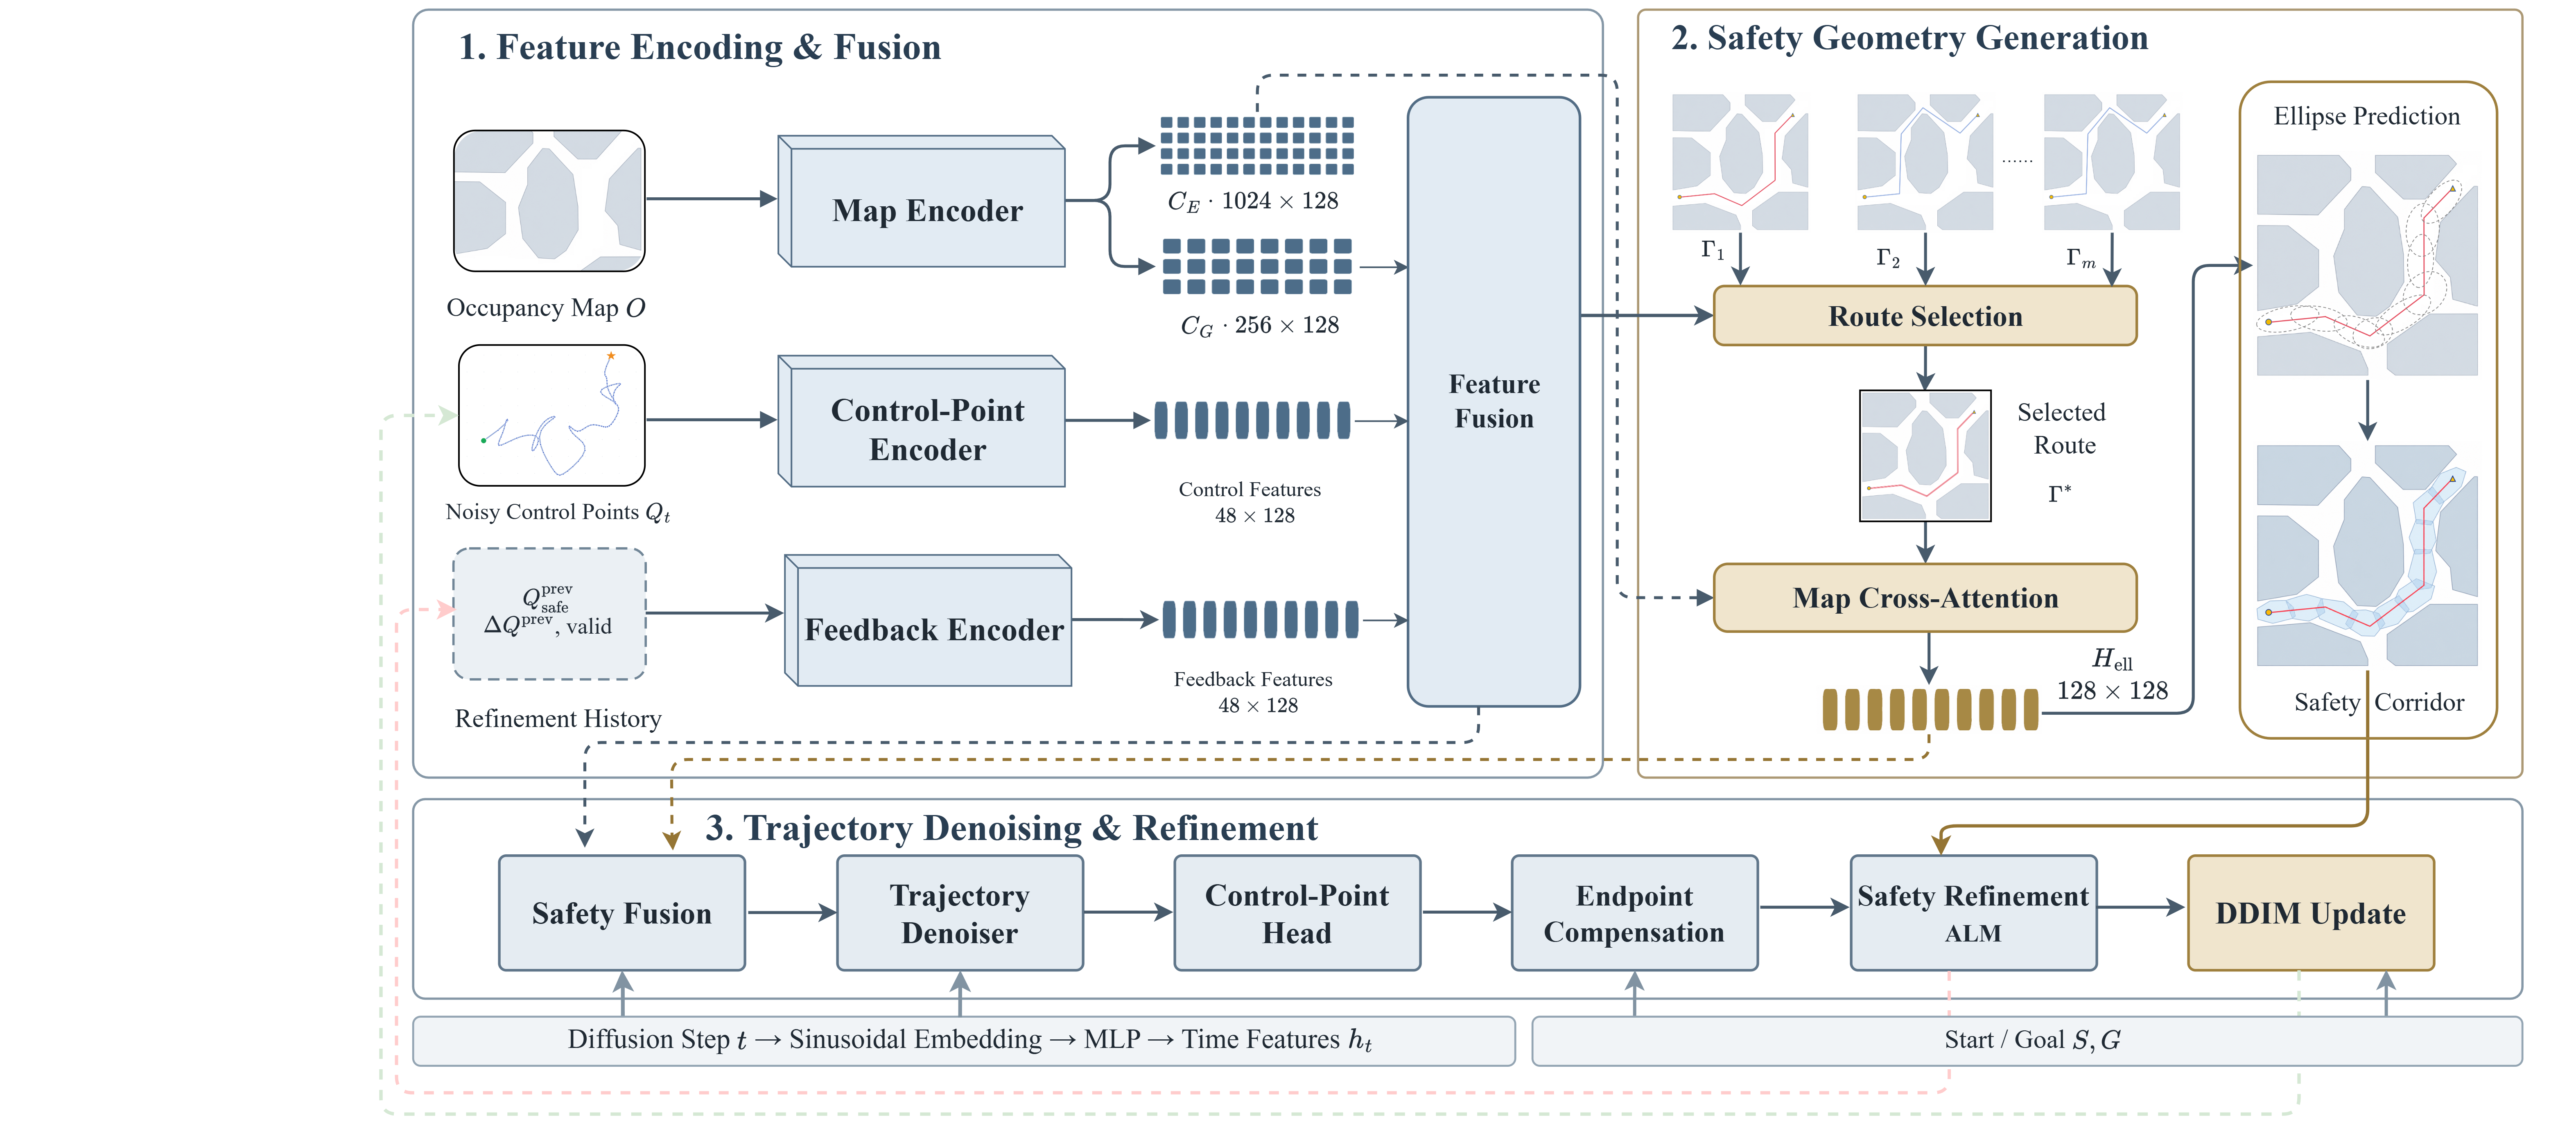
\includegraphics[width=0.85\textwidth]{fig1_framework.png}
\caption{Overall framework of TrajSafe-Diffuser.}
\label{fig:framework}
\end{figure*}

As shown in Fig.~\ref{fig:framework}, the method consists of three parts: feature encoding and fusion, safety feature and constraint generation, and trajectory denoising and safety correction. The occupancy map, the noisy control points and the historical correction are encoded and fused, and the result is used for candidate route matching; the local safety geometry is predicted along the selected route, and the safety latent features used for denoising together with the convex safe corridor used for constraint correction are generated. After endpoint compensation and correction by the augmented Lagrangian method (ALM), the denoising prediction influences the subsequent sampling through the DDIM state update and the historical feedback.

\subsection{Feature Encoding and Fusion}
\label{sec:feature}

\subsubsection{Map and Control Point Feature Encoding}

The map encoder extracts a global map memory $C_G\in\R^{256\times128}$ and a local map memory $C_E\in\R^{1024\times128}$, corresponding to spatial resolutions of $16\times16$ and $32\times32$, respectively, with spatial positional encodings added. The former participates in control point encoding and denoising, whereas the latter is used for safety geometry queries. The noisy control points $q_{t,j}$ are mapped by a coordinate encoding and an MLP and then added to the control point index encoding, giving
\begin{equation}
X_j^{(0)}
=\MLP_T\bigl(\Phi_{xy}(q_{t,j})\bigr)
+\PE_{1D}(j),
\end{equation}
where $\Phi_{xy}$ and $\PE_{1D}$ provide spatial position and control point order information, respectively.

\begin{figure}[!t]
\centering
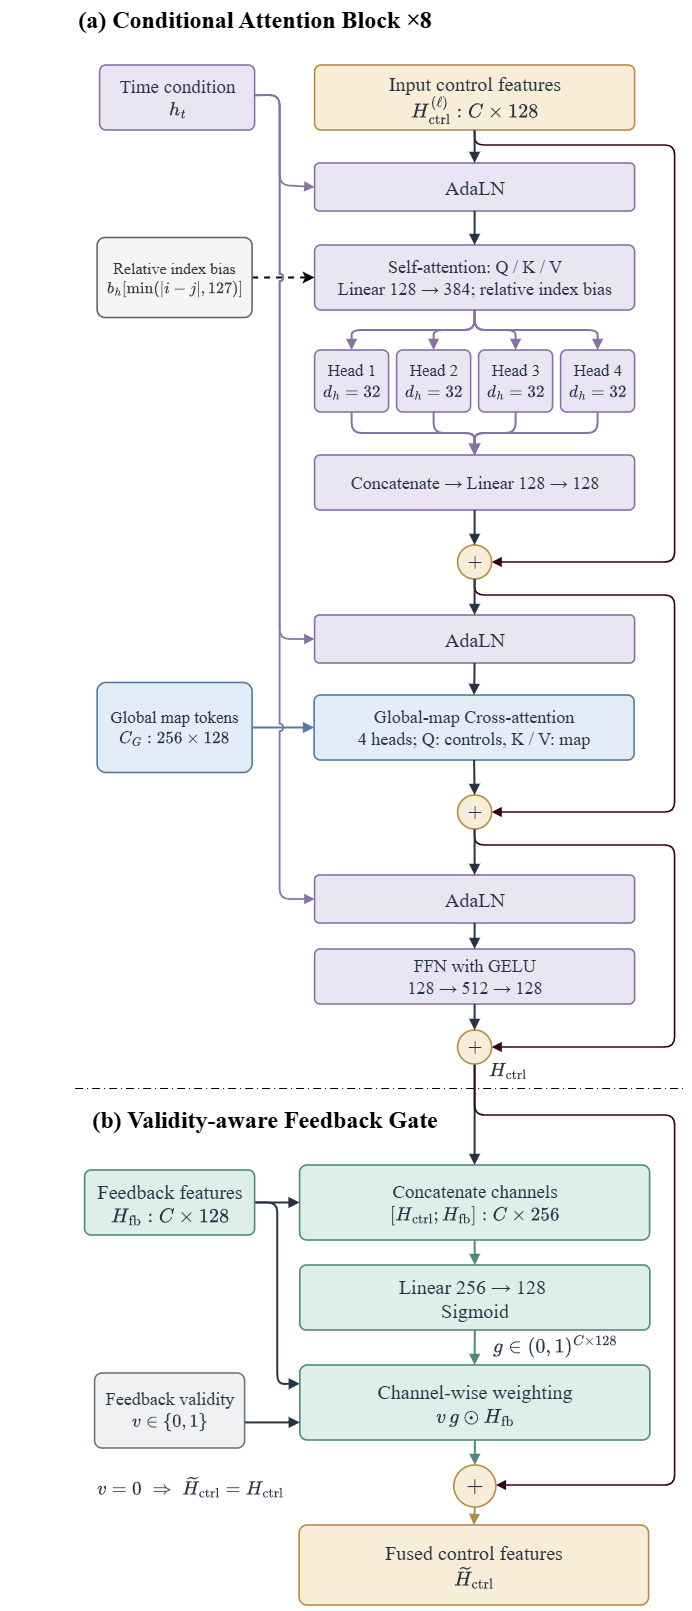
\includegraphics[width=0.70\columnwidth]{fig2_feature_fusion.png}
\caption{Conditional attention and historical-feedback gated fusion. (a) The conditional attention block consists of control point self-attention, global-map cross-attention and a feed-forward network, and extracts control features through time-condition modulation and residual connections. (b) Historical safety correction features are fused into the current control features through a feedback validity flag and channel-wise gating.}
\label{fig:fusion}
\end{figure}

As shown in Fig.~\ref{fig:fusion}(a), the control features pass through eight conditional attention blocks, each of which contains control point self-attention, map cross-attention with $C_G$ as keys and values, and a feed-forward network, all with residual connections. The number of attention heads is 4 and the feature dimension is 128. The time step $t$ is mapped to $h_t$ by sinusoidal encoding and an MLP, and modulates each sublayer through adaptive layer normalization:
\begin{equation}
\Ada(X,h_t)
=\bigl(1+\gamma(h_t)\bigr)\odot\LN(X)
+\beta(h_t),
\end{equation}
where $\gamma$ and $\beta$ are the channel-wise scaling and shifting parameters generated from the time condition. The encoding output is $H_{\mathrm{ctrl}}\in\R^{48\times128}$.

\subsubsection{Historical Safety Feedback Fusion}

To exploit previous trajectory correction results, the most recent control points $Q_{\mathrm{hist}}$ that passed the acceptance check, the correction $\Delta Q_{\mathrm{hist}}$ and a validity flag $v\in\{0,1\}$ are used as feedback inputs. The five-dimensional vector of each control point is encoded by a $5\!\rightarrow\!64\!\rightarrow\!128$ MLP into $H_{\mathrm{fb}}\in\R^{48\times128}$. The channel-wise gating in Fig.~\ref{fig:fusion}(b) is
\begin{equation}
\begin{aligned}
g&=\sigma\bigl(W_g[H_{\mathrm{ctrl}};H_{\mathrm{fb}}]+b_g\bigr),\\
\widetilde H_{\mathrm{ctrl}}
&=H_{\mathrm{ctrl}}+v\,g\odot H_{\mathrm{fb}},
\end{aligned}
\end{equation}
where $[\cdot;\cdot]$ denotes channel concatenation, $\sigma$ is the sigmoid function and $g\in\R^{48\times128}$. When $v=0$, the feedback branch does not change the current control features; valid feedback is injected adaptively per control point and per channel. The fused result $\widetilde H_{\mathrm{ctrl}}$ is used for route matching and conditioned denoising.

\subsection{Safety Feature and Constraint Generation}

In this subsection, route matching and local geometry prediction are illustrated in Fig.~\ref{fig:route} and Fig.~\ref{fig:geom}, respectively.

% \subsubsection{Route Matching and Selection}

% At most $M$ candidate routes $\{\Gamma_m\}_{m=1}^{M}$ are extracted from free space and encoded after equal-arclength resampling to give $H_{S,m}\in\R^{128\times128}$. As shown in Fig.~\ref{fig:route}, time-conditioned cross-attention is performed with $\widetilde H_{\mathrm{ctrl}}$ as queries and $H_{S,m}$ as keys and values, and matching features $R_m\in\R^{48\times128}$ are obtained through a feed-forward residual module. After average pooling over the control point dimension, a scoring head produces $\ell_m$, and on the set of valid candidates $\mathcal V$,
% \begin{equation}
% \pi_m=\frac{\exp(\ell_m)}{\sum_{k\in\mathcal V}\exp(\ell_k)},
% \qquad m\in\mathcal V.
% \end{equation}
% The candidate with the highest score is selected first; if its safe corridor fails to be constructed, the remaining candidates are tried in turn. Once the corridor is successfully activated, the selected route $\Gamma^*$ and its feature $H_S^*$ are fixed, which avoids inconsistency between the route and the constraint during subsequent sampling.

% \begin{figure}[!t]
% \centering
% 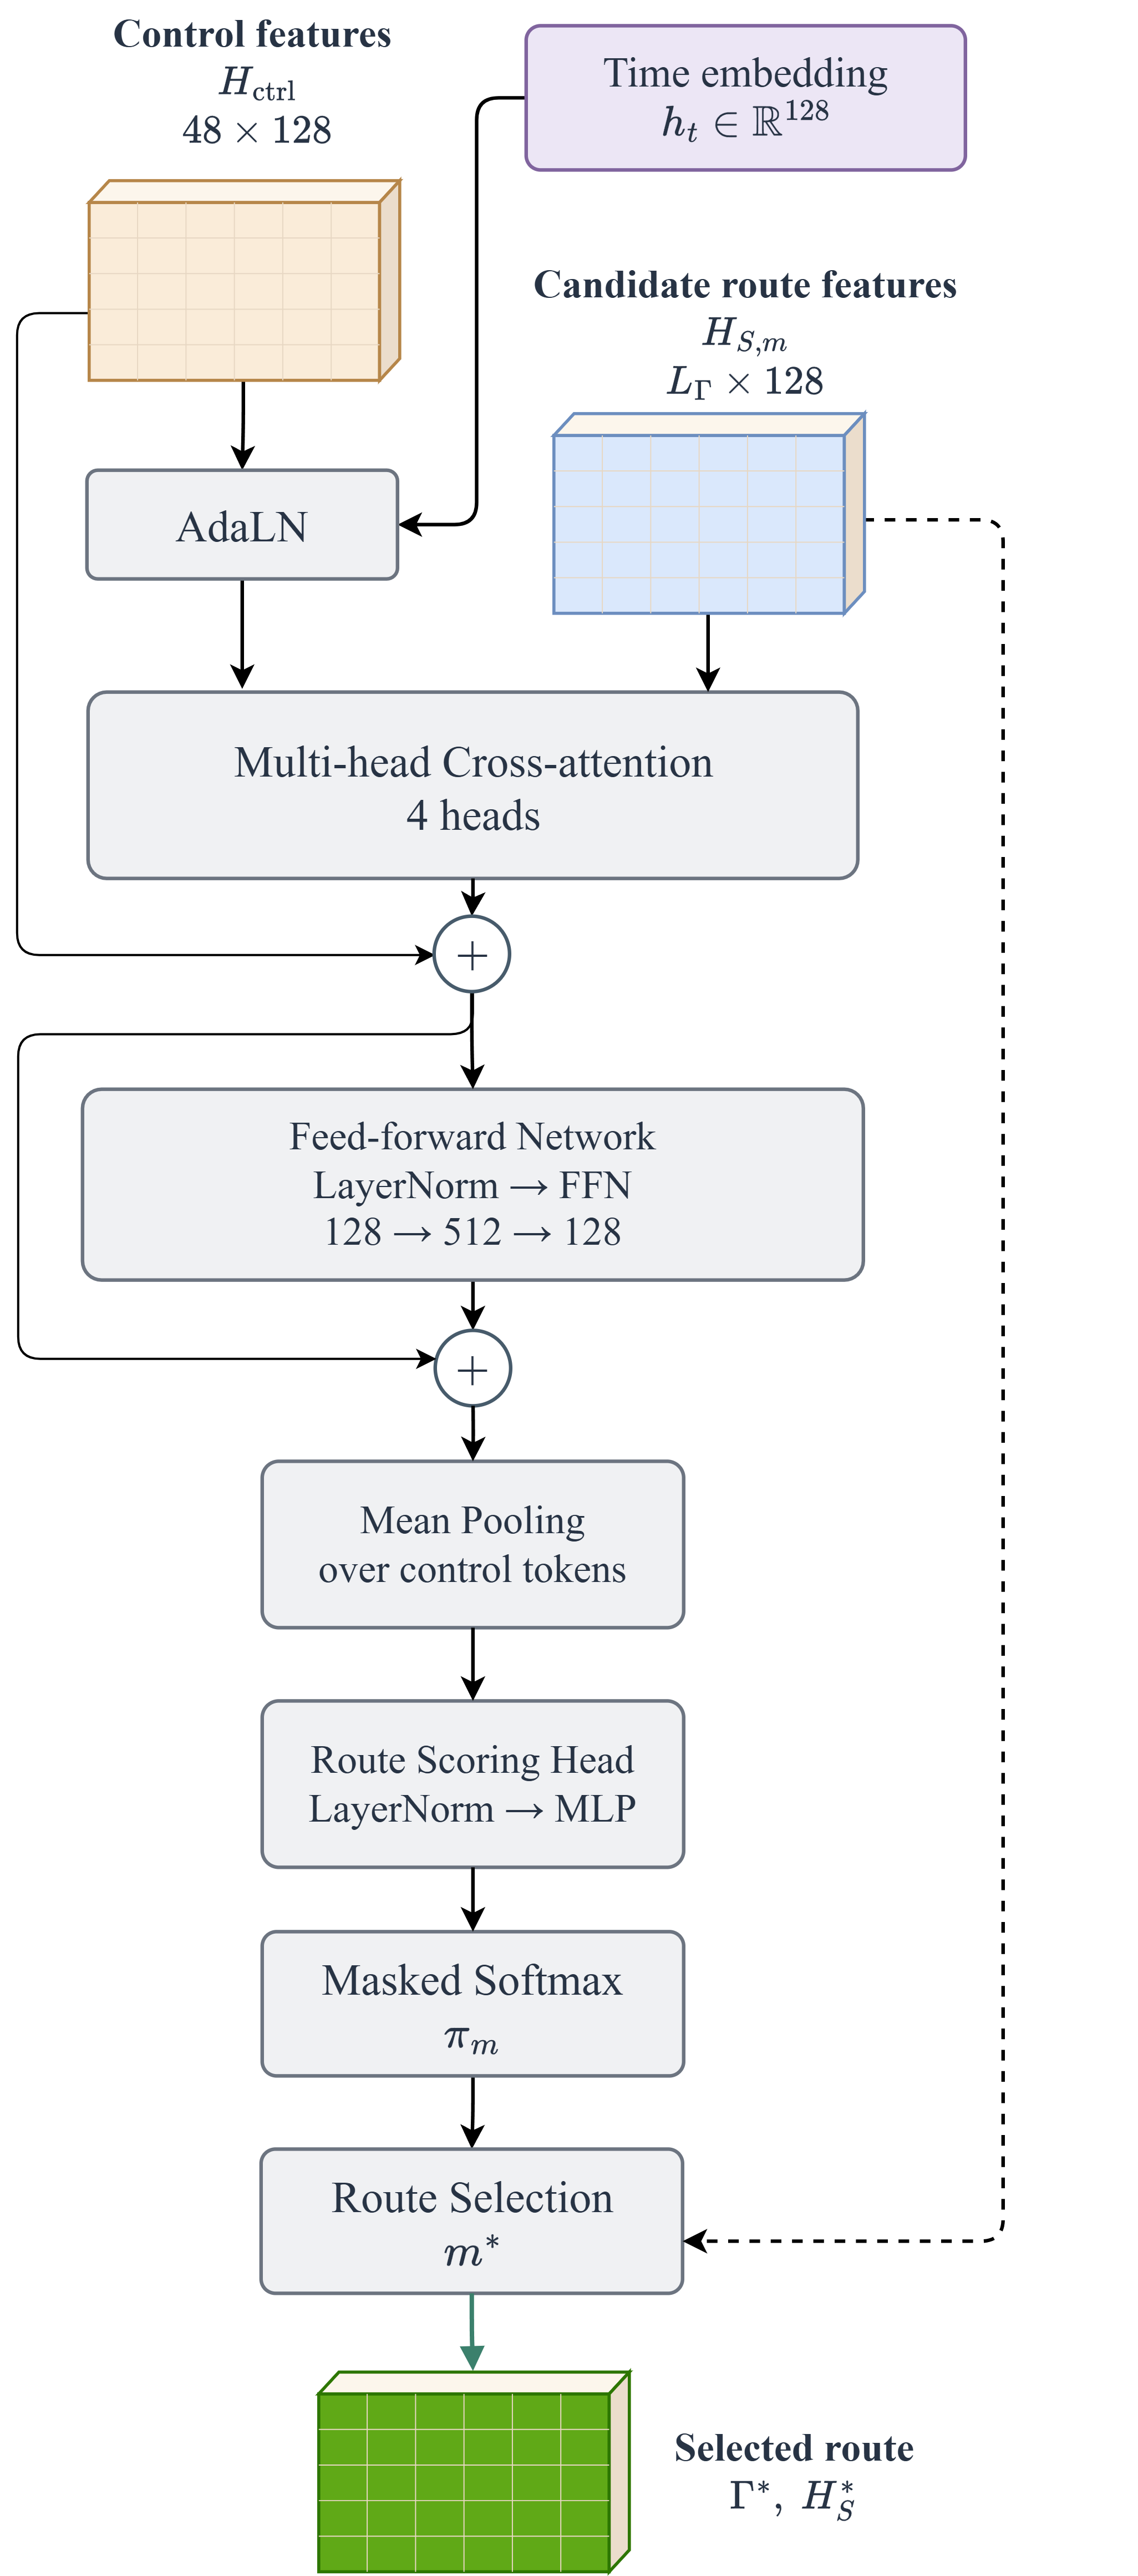
\includegraphics[width=0.90\columnwidth]{fig3a_route_selection.png}
% \caption{Candidate route matching and selection. The fused control features serve as queries and the candidate route features as keys and values; a time-modulated cross-attention block together with a feed-forward residual module forms the matching features, and average pooling, a scoring head and a masked softmax select the task-relevant route.}
% \label{fig:route}
% \end{figure}

\subsubsection{Local Safety Geometry Prediction}

$N_q=128$ fixed safety centers $c_i=\Gamma^*\!\left(i/(N_q-1)\right)$ are sampled at equal arclength along $\Gamma^*$. The network predicts only the scale and orientation of the corresponding ellipse, which avoids the obstacle intrusion and convex region construction failure that direct regression of the center positions may cause. The selected route feature forms $H_\Gamma\in\R^{128\times128}$ through the safety query network and queries the local map memory $C_E$. To prioritize the obstacle structure near the center, a spatial bias is added to the pre-normalization score of every attention head:
\begin{equation}
\begin{aligned}
\mathcal B_{ij}^{\mathrm{geo}}&=\clip\!\left(
-\frac{\baralpha_t\|c_i-z_j\|_2^2}{2\sigma_{\mathrm{geo}}^2},
-b_{\mathrm{clip}},0\right),\\
w_{ij}&=\softmax_j\!\left(
\frac{q_i^{\top}k_j}{\sqrt{d_h}}+\mathcal B_{ij}^{\mathrm{geo}}\right).
\end{aligned}
\end{equation}
where $z_j$ is the spatial position of the map token, $q_i,k_j$ are the projected query and key vectors and $d_h$ is the single-head dimension; $\sigma_{\mathrm{geo}}$ and $b_{\mathrm{clip}}$ control the distance decay scale and the clipping range, respectively. As $\baralpha_t$ increases during the reverse diffusion, the distance bias strengthens the local query. The resulting safety features are
\begin{equation}
H_{\mathrm{ell}}
=H_\Gamma+\CA_{\mathcal B^{\mathrm{geo}}}
\bigl(\Ada(H_\Gamma,h_t),C_E\bigr).
\end{equation}
The ellipse shape head predicts $e_i=(\log a_i,\log b_i,\cos2\theta_i,\sin2\theta_i)$ from $H_{\mathrm{ell}}\in\R^{128\times128}$, which together with the fixed center $c_i$ determines the local ellipse. \textbf{The predicted ellipse only provides a geometric scale and orientation prior and does not directly guarantee obstacle avoidance.} Subsequently, with the complete obstacle grid cells and the map boundary as constraints, a deterministic geometric constructor combines a safety margin and geometric separation to form convex safe regions
\begin{equation}
\mathcal R_i=\{x\in\R^2\mid A_ix\leq b_i\},
\end{equation}
where $A_i,b_i$ are the half-space parameters. The constructor checks the intersection of the regions with obstacles and the overlap between adjacent regions, adding bridging regions when necessary, to obtain an ordered convex safe corridor $\mathcal C$. Therefore, the $H_{\mathrm{ell}}$ and $\mathcal C$ generated from the same route provide the learned denoising condition and the explicit trajectory constraint, respectively.


\begin{figure*}[!t]
\centering
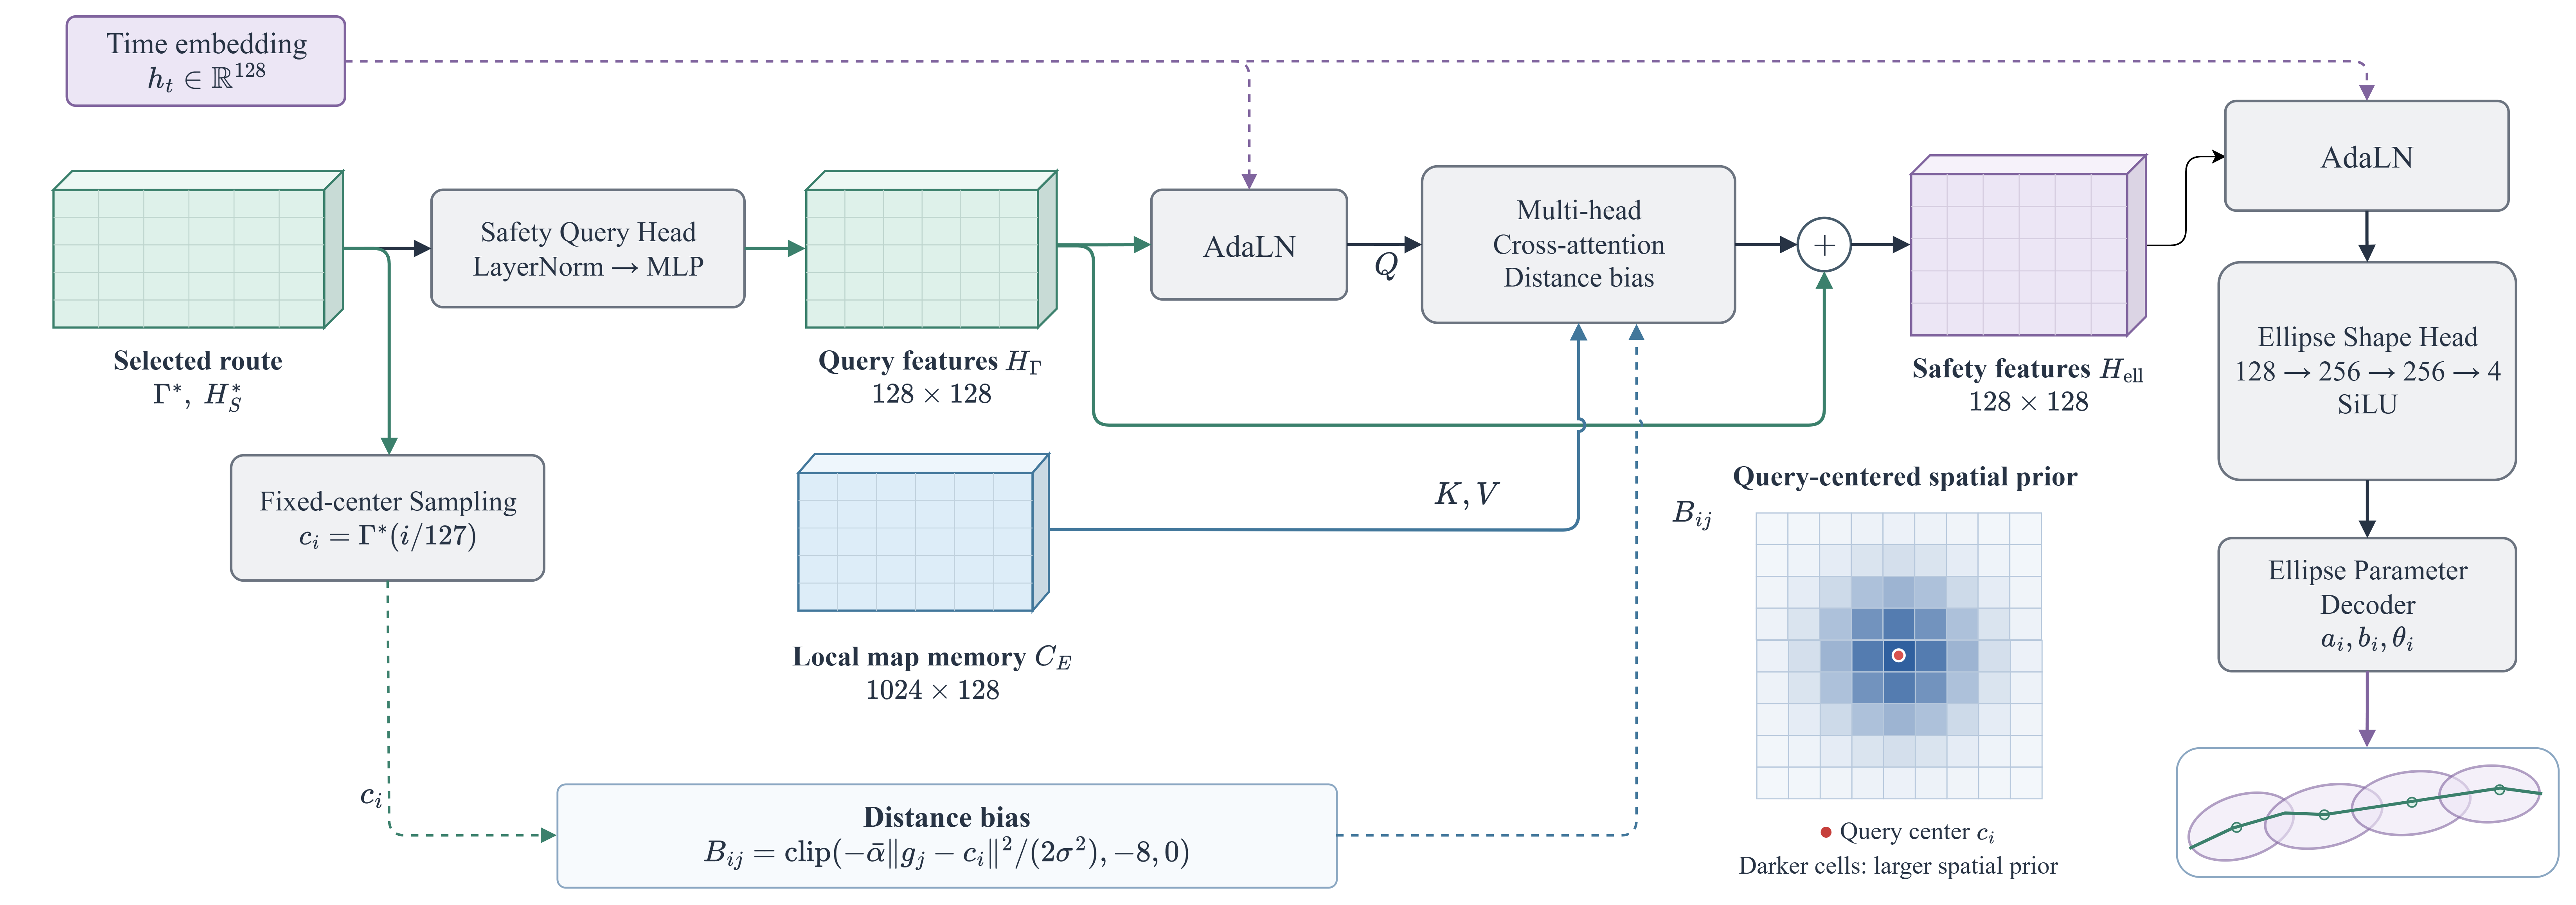
\includegraphics[width=0.85\textwidth]{fig3b_safety_geometry.png}
\caption{Local safety feature and ellipse geometry prediction. Safety centers are sampled at fixed positions along the selected route, and a spatial distance bias between the centers and the map positions is added to the cross-attention; the resulting safety latent features are passed through an ellipse shape head that outputs the local semi-axes and orientation, which are used for the subsequent convex safe region construction.}
\label{fig:geom}
\end{figure*}

% \subsection{Trajectory Denoising and Safety Correction}
% \label{sec:denoise}

% \subsubsection{Safety-Conditioned Denoising and Endpoint Compensation}

% As shown in the upper part of Fig.~\ref{fig:denoise}, $\widetilde H_{\mathrm{ctrl}}$ serves as queries to read the safety features $H_{\mathrm{ell}}$ through four-head cross-attention, and $F\in\R^{48\times128}$ is formed by residual fusion and an MLP. Clean control points $\widehat Q_{0,\mathrm{raw}}^{(t)}$ are then predicted by three conditional denoising blocks with independent parameters, conditioned on the global map memory $C_G$ and the time feature $h_t$. The single-block denoising module is shown in the lower part of Fig.~\ref{fig:denoise}; its self-attention, map cross-attention and feed-forward structures are identical in form to the conditional attention encoding of Section~\ref{sec:feature} and are not repeated here.

% \begin{figure*}[!t]
% \centering
% 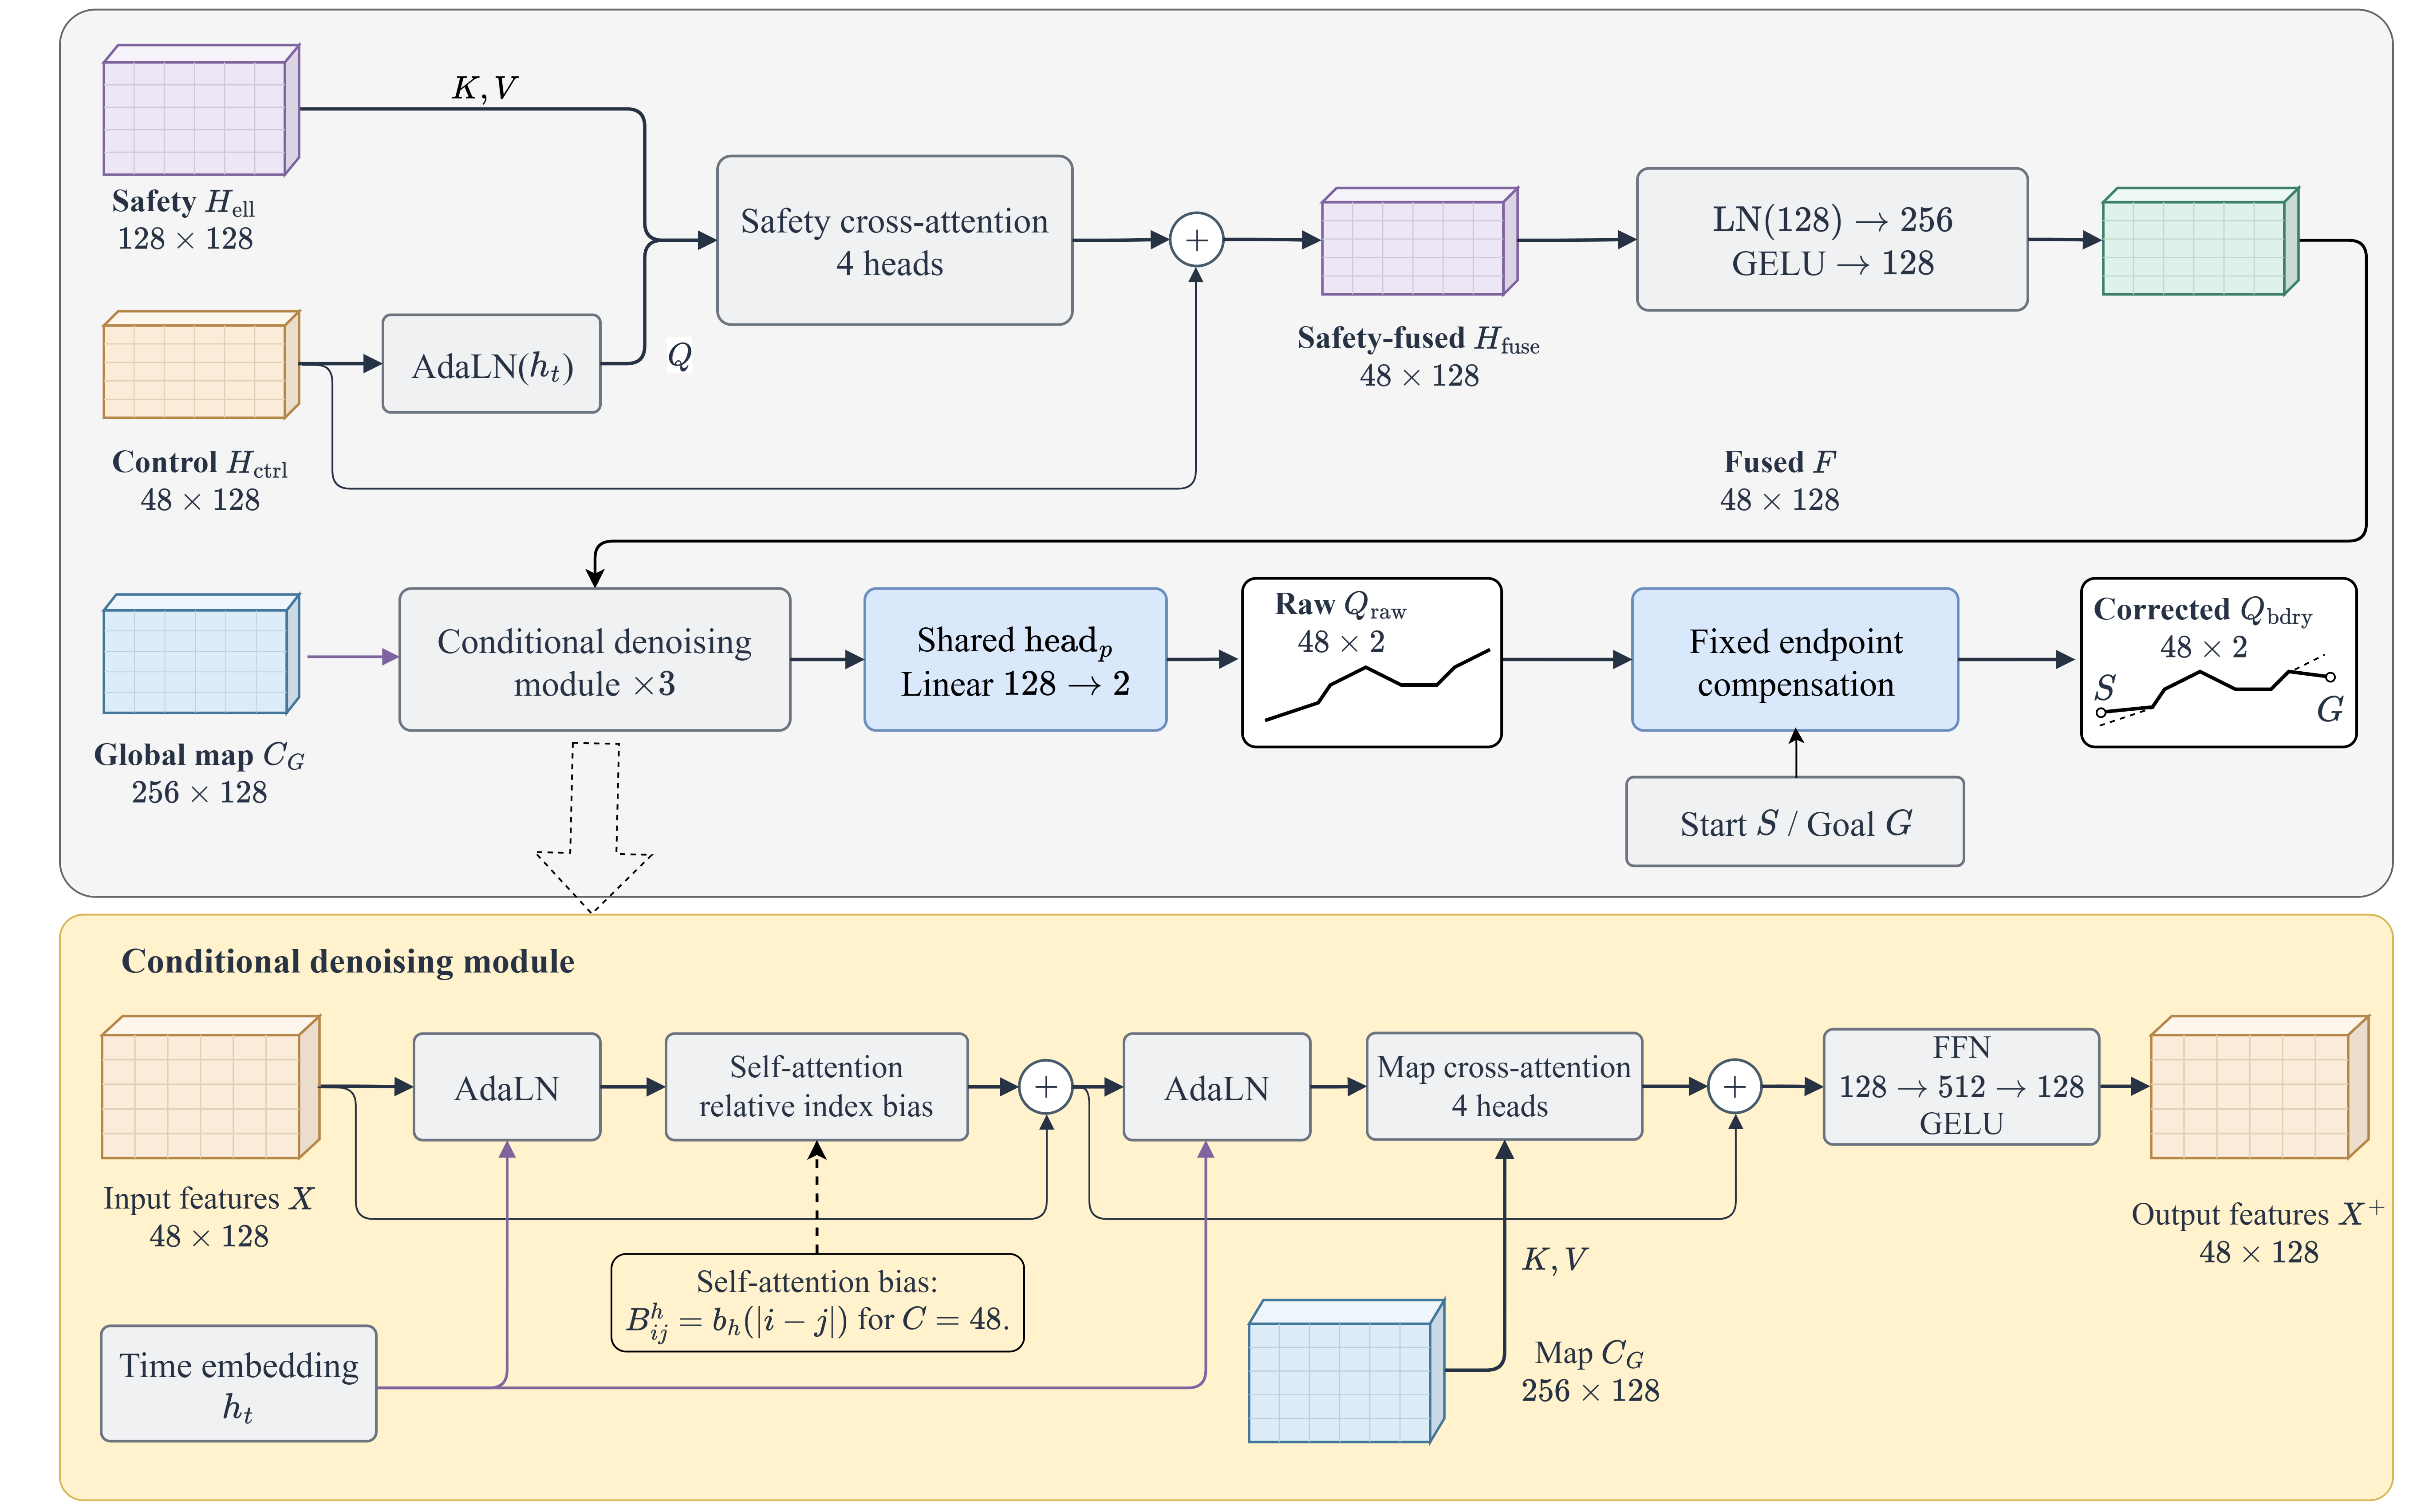
\includegraphics[width=0.85\textwidth]{fig4_denoising.png}
% \caption{Safety-conditioned denoising and control point prediction. Upper: the control features read the local safety latent features through cross-attention, and the fused features pass through three conditional denoising blocks, a coordinate prediction head and endpoint compensation to yield control points that satisfy the start and goal position constraints. Lower: single conditional denoising block, in which the diffusion time condition is injected through AdaLN, followed by control point self-attention, global-map cross-attention and a feed-forward transformation, with residual connections applied to all three sublayers.}
% \label{fig:denoise}
% \end{figure*}

% To satisfy the fixed start and goal and to alleviate the local deformation caused by directly replacing the endpoints, the first and last prediction errors are compensated to the neighbouring control points with fixed weights:
% \begin{equation}
% \widehat q_{0,\mathrm{bdry},j}^{(t)}
% =\widehat q_{0,\mathrm{raw},j}^{(t)}
% +w_j^S\bigl(S-\widehat q_{0,\mathrm{raw},0}^{(t)}\bigr)
% +w_j^G\bigl(G-\widehat q_{0,\mathrm{raw},C-1}^{(t)}\bigr),
% \end{equation}
% where $w_j^S,w_j^G$ are fixed weights in the neighbourhoods of the start and the goal satisfying $w_0^S=w_{C-1}^G=1$ and $w_0^G=w_{C-1}^S=0$, which guarantees that the two end points after compensation are $S$ and $G$, respectively. The resulting control points are denoted by $\widehat Q_{0,\mathrm{bdry}}^{(t)}$.

% \subsubsection{Continuous-Trajectory Safety Constraints and ALM Correction}

% To constrain the whole continuous curve, the B-spline knot intervals and the responsibility intervals of the safe regions are jointly subdivided, and each subinterval is converted into cubic B\'ezier form. The four control points of the $\ell$-th segment satisfy
% \begin{equation}
% \beta_\ell=E_\ell Q,
% \qquad E_\ell\in\R^{4\times48}.
% \end{equation}
% By the B\'ezier convex hull property, as long as the four control points of each segment lie in the assigned convex region $\mathcal R_{j(\ell)}$, the whole corresponding curve segment lies in that region. The continuous safety condition can therefore be sufficiently guaranteed by linear inequalities on the original B-spline control points:
% \begin{equation}
% g_{\ell,r,f}(Q)
% =a_{j(\ell),f}^{\mathsf T}(E_\ell Q)_r
% -b_{j(\ell),f}\leq0,
% \quad r=0,1,2,3,
% \end{equation}
% where $f$ is the half-space index of the convex region; the collected constraints are denoted by $g(Q)\leq0$, without introducing additional independent B\'ezier optimization variables.

% \begin{figure}[!t]
% \centering
% 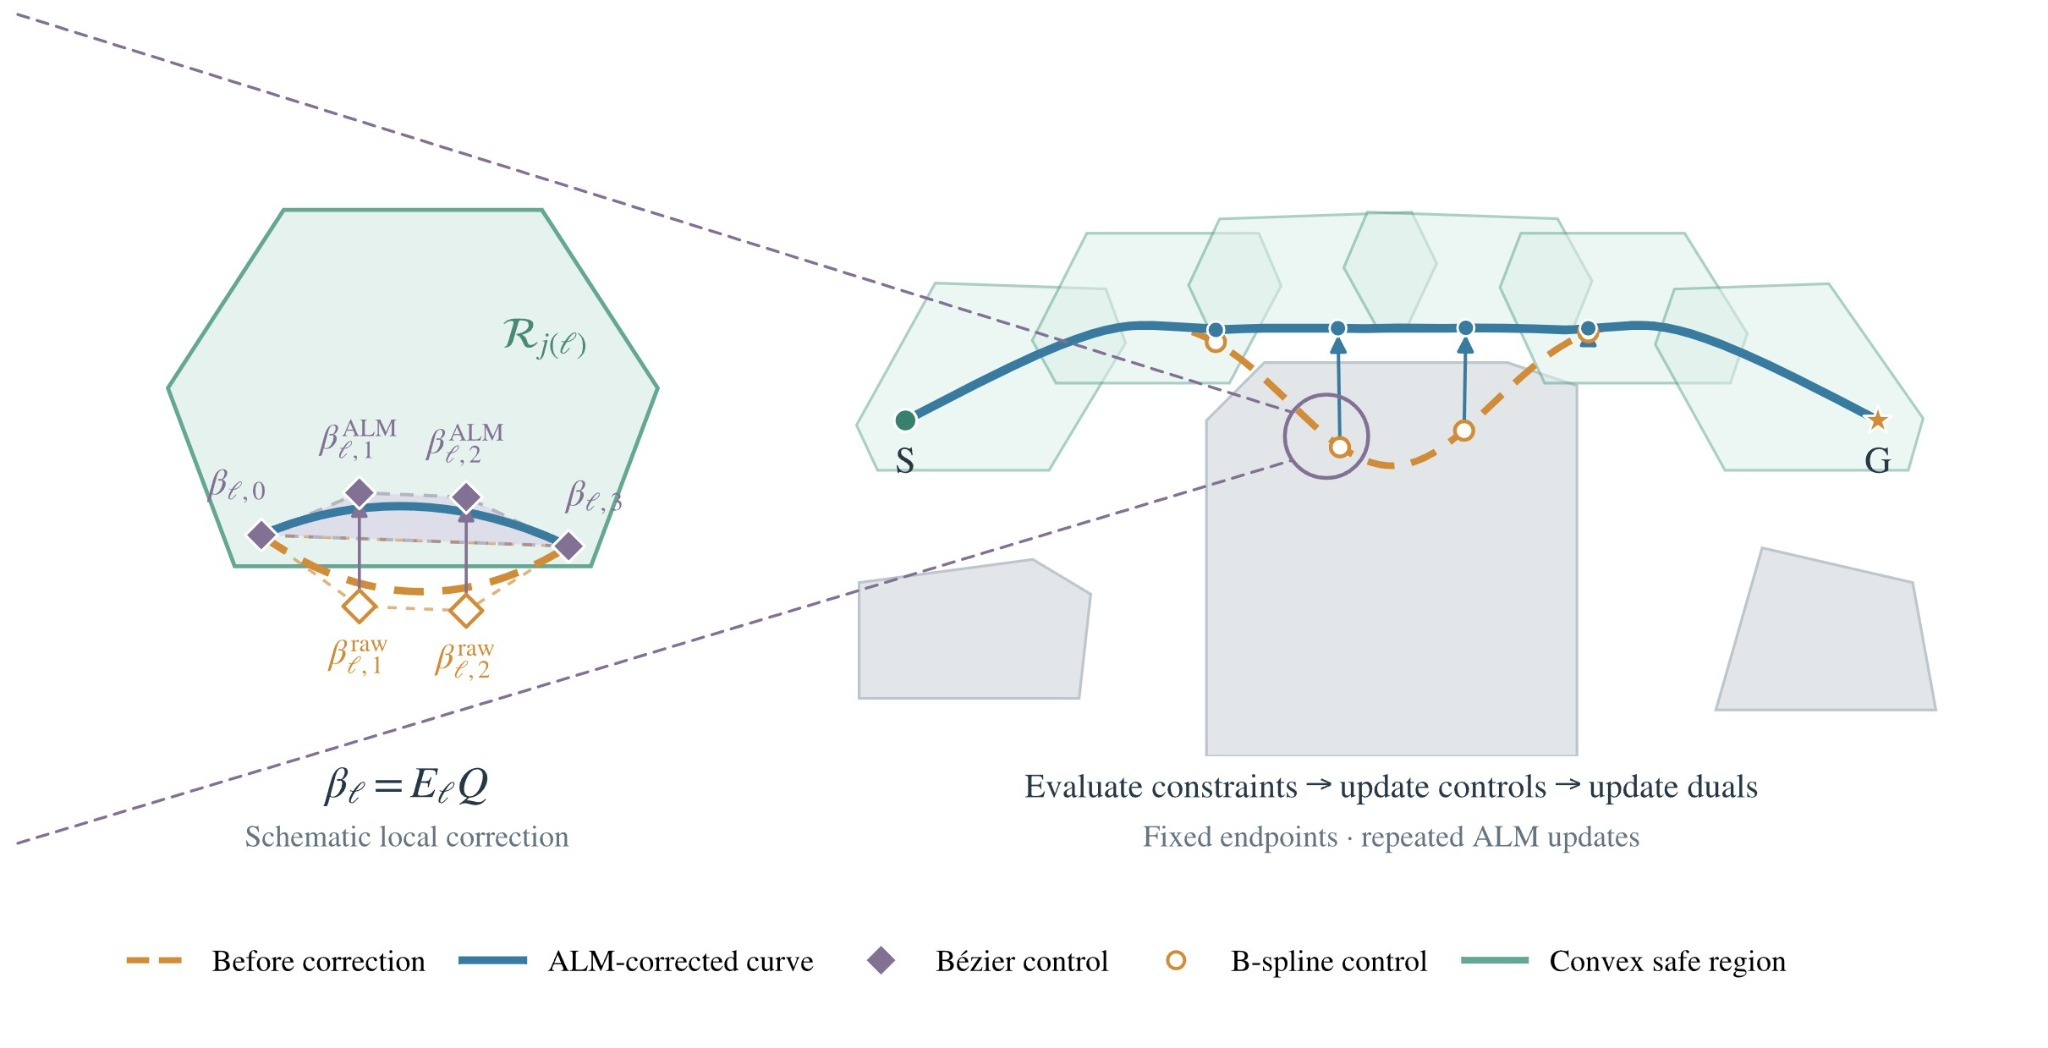
\includegraphics[width=\columnwidth]{fig5_alm_constraint.jpg}
% \caption{Illustration of the continuous-curve safety constraint and the augmented Lagrangian control point correction. Right: change of the predicted trajectory and of the B-spline control points after the ALM correction under fixed start and goal; left: zoom of a local B\'ezier curve and its control points, illustrating the relation between the control point constraints and the membership of the convex region.}
% \label{fig:alm}
% \end{figure}

% As shown in Fig.~\ref{fig:alm}, with $Q^{\mathrm{ref}}=\widehat Q_{0,\mathrm{bdry}}^{(t)}$ as a reference, ALM is used to solve
% \begin{equation}
% \begin{aligned}
% \min_{Q}\quad
% &J(Q-Q^{\mathrm{ref}})=
% \frac{\lambda_p}{2}\bigl\|B(Q-Q^{\mathrm{ref}})\bigr\|_F^2\\
% &\qquad
% +\frac{\lambda_s}{2}\bigl\|D_2B(Q-Q^{\mathrm{ref}})\bigr\|_F^2,\\
% \mathrm{s.t.}\quad
% &g(Q)\leq0,\quad q_0=S,\quad q_{C-1}=G,
% \end{aligned}
% \end{equation}
% where $B$ is the B-spline sampling basis matrix and $D_2$ is the second-order difference operator; the two terms suppress the trajectory offset and the shape change after correction, respectively. Introducing non-negative multipliers $\mu$ and a penalty coefficient $\rho$, the augmented Lagrangian function is
% \begin{equation}
% \mathcal L_\rho(Q,\mu)
% =J(Q-Q^{\mathrm{ref}})
% +\frac{\bigl\|[\mu+\rho g(Q)]_+\bigr\|_2^2-\|\mu\|_2^2}{2\rho},
% \end{equation}
% where $[\cdot]_+$ denotes the element-wise positive part. During the optimization the internal control points and the multipliers are updated alternately while the end points are kept fixed. After a finite number of iterations yields $Q_{0,\mathrm{ALM}}^{(t)}$, a constraint residual check is performed; the B\'ezier convex hull condition is a sufficient condition for continuous containment, but whether the output of the finite-iteration optimization satisfies it still needs to be confirmed by the actual residual.


% \subsubsection{Safety State Update and Historical Feedback}

% The safety correction influences the subsequent reverse diffusion through two paths. First, the noise is recomputed with $Q_{0,\mathrm{ALM}}^{(t)}$ and a deterministic DDIM update is performed:
% \begin{equation}
% \begin{aligned}
% \widehat\epsilon_t&=
% \frac{Q_t-\sqrt{\baralpha_t}\,Q_{0,\mathrm{ALM}}^{(t)}}{\sqrt{1-\baralpha_t}},\\
% Q_s&=\sqrt{\baralpha_s}\,Q_{0,\mathrm{ALM}}^{(t)}
% +\sqrt{1-\baralpha_s}\,\widehat\epsilon_t,
% \qquad s<t.
% \end{aligned}
% \end{equation}
% The first and last control points are still fixed after the update. Second, for results that pass the acceptance check, $Q_{\mathrm{hist}}=Q_{0,\mathrm{ALM}}^{(t)}$ and $\Delta Q_{\mathrm{hist}}=Q_{0,\mathrm{ALM}}^{(t)}-\widehat Q_{0,\mathrm{bdry}}^{(t)}$ are cached and participate in the next feature fusion in the gated manner of Section~\ref{sec:feature}. If the correction fails the acceptance check, the existing valid history is not overwritten. The DDIM path directly changes the subsequent sampling state, while the historical feedback path provides the previous correction information to the next network prediction.

% \subsection{Training Strategy and Loss Function}
% \label{sec:loss}

% \subsubsection{Two-Forward Training with Shared Parameters}

% To enable the network to exploit the historical safety correction information in the reverse diffusion process, this paper adopts a two-forward training strategy with shared parameters. First, a diffusion time step $t$ is randomly sampled, noise is added to the reference control points to obtain $Q_t$, and a first network forward pass is performed without historical feedback to predict the clean control points. The offline convex safe corridor corresponding to the reference route is then used for ALM correction, and the historical correction control points, the correction and the validity flag are constructed from the constraint residual check. When the raw prediction already satisfies the constraints, the feedback correction is set to zero; when the correction result fails the check, the feedback flag is set to invalid. One DDIM update is performed with the corrected control points to obtain the state $Q_s$ at the adjacent time step $s=t-1$.

% The second forward pass receives $Q_s$ and the constructed historical feedback and predicts the clean control points again with the same network parameters. The ALM solve, the constraint check, the feedback construction and the DDIM state update all stop gradient propagation, so that the gradients of the second prediction do not back-propagate to the first prediction through the above process. During training the historical feedback is randomly masked with a probability of 25\%, so as to accommodate the situation at the beginning of inference where no valid feedback is available yet.

% \subsubsection{Loss Function}

% To simultaneously optimize the trajectory prediction accuracy, the safety geometry representation and the degree of trajectory constraint satisfaction, this paper uses three categories of losses: trajectory prediction, safety geometry and safety constraints.

% \emph{Trajectory prediction losses:} these include the control point reconstruction loss $\mathcal L_{\mathrm{ctrl}}$, the boundary loss $\mathcal L_{\mathrm{boundary}}$ and the control point smoothness loss $\mathcal L_{\mathrm{smooth}}$. The control point reconstruction loss computes the mean squared error between the predicted internal control points and the reference control points. The boundary loss constrains the shape of the control points near the start and the goal. Specifically, the reference control point set is translated so that its start or its goal aligns with the current planning task, giving two sets of local reference control points; a weighted squared error between the predicted control points and the corresponding reference control points is then computed, with weights that decrease as the control points move away from the start and the goal. This loss mainly limits the change of the trajectory shape near the endpoints, whereas the start and goal position constraints are satisfied directly by the endpoint compensation mechanism. The control point smoothness loss measures the local shape change by the second- and third-order differences of the predicted control points, normalized by the average spacing of the reference control points to reduce the influence of different trajectory scales.

% \emph{Safety geometry losses:} these include the route classification loss $\mathcal L_{\mathrm{topo}}$, the ellipse shape loss $\mathcal L_{\mathrm{shape}}$, the region overlap loss $\mathcal L_{\mathrm{IoU}}$ and the ellipse safety loss $\mathcal L_{\mathrm{safe}}$. The route classification loss uses cross-entropy to supervise candidate route selection, and its supervision label is determined by the normalized dynamic time warping distance between the reference trajectory and the candidate routes. The ellipse shape loss uses the mean squared error to constrain the predicted log-semi-axes and double-angle orientation parameters; the region overlap loss measures the spatial coverage difference by the intersection over union between the predicted ellipse and the reference ellipse soft raster mask. The ellipse safety loss is computed from the overlap ratio between the predicted ellipse and the obstacle regions, combining the mean intrusion ratio with the mean intrusion degree of the most severe 20\% of the regions, so as to reduce the obstacle occupancy risk of the local safety geometry.

% \emph{Safety constraint losses:} these include the corridor loss $\mathcal L_{\mathrm{alm}}$ and the continuous safety loss $\mathcal L_{\mathrm{fb,safe}}$. The corridor loss acts on the trajectory sample points obtained by decoding the first prediction, computes the degree of constraint violation of the sample points with respect to the valid convex safe corridor, and penalizes violations exceeding the tolerance. The continuous safety loss acts on the prediction of the second forward pass and computes the maximum positive residual over all constraints using the B\'ezier control point inequalities defined in Section~\ref{sec:denoise}. Unlike the corridor loss, which is based on discrete trajectory sample points, the continuous safety loss directly constrains the B\'ezier control points in order to reduce the continuous-curve constraint violation of the second prediction. In addition, the second forward pass also uses a curve smoothness loss $\mathcal L_{\mathrm{curve}}$, which imposes second- and third-order difference penalties on the decoded B-spline curve.

\section{Experiments and Analysis}
%=====================================================================

\subsection{Experimental Setup}

\subsubsection{Dataset and Implementation Details}

The experiments use a two-dimensional static occupancy grid trajectory dataset built from CARLA road scenes~\cite{dosovitskiy2017carla}. Each scene covers $160\,\mathrm{m}\times160\,\mathrm{m}$, the map size is $256\times256$ and the spatial resolution is $0.625\,\mathrm{m/grid}$; obstacles are dilated by $4$ grid cells and the map boundary is treated as an impassable region. The training set consists of 3850 samples from Town03 and Town04, the validation set contains 1550 samples from Town05, and the test set contains 420 samples from Town01, Town02 and Town10HD, with the test towns excluded from training. Quality evaluation for the main comparison, the ablation and the acceleration configurations all uses the same test set and random seeds 0, 1 and 2, and 1260 trajectories are generated for each configuration.

All models use a cubic B-spline representation with 48 control points and are trained for 200 epochs on an NVIDIA GeForce RTX 4070 with a learning rate of $2\times10^{-4}$ and a batch size of 16. In order to distinguish the safety condition from the feedback mechanism, three generators are used: D is the base diffusion model, which does not contain the safety condition or the historical feedback; S additionally introduces the safety condition and geometric supervision but does not use feedback training; A adopts the two-forward feedback training of Section~\ref{sec:loss} on top of the safety condition. All three select the model weights according to the task score on the validation set, and the test set does not participate in model selection.

Standard inference uses 16 DDIM steps, the first 3 forward passes serve as warm-up, after which the safe corridor is activated and the ALM correction is performed; the first correction runs at most 8 inner iterations and the subsequent ones at most 10. The 4-step configuration shortens the warm-up to 2 passes while keeping the remaining optimization settings unchanged. Trajectory collisions and corridor responsibility-region residuals are both evaluated by sampling 512 equally spaced points along the continuous curve. It should be noted that this discrete check cannot replace a continuous safety verification of the inequalities of all B\'ezier control points.

\subsubsection{Comparison Methods and Evaluation Metrics}

In order to examine the effect of explicit safety constraints, four baselines are set up: unconstrained diffusion, fixed-penalty guidance, primal-dual guidance and SDF augmented Lagrangian guidance. Unconstrained diffusion outputs the generated trajectory directly; fixed-penalty guidance corrects the control points along the gradient of the collision cost of the signed distance field (SDF); primal-dual guidance alternately updates the control variables and the constraint multipliers; and SDF augmented Lagrangian guidance further introduces a quadratic violation penalty term. All four baselines use generator D and the same initial noise, the parameters of the three SDF-based guidance variants are selected on the validation set, and the inner iteration limit is 10 for all of them. The complete TrajSafe-Diffuser uses generator A together with the convex safe corridor, the ALM correction and the historical feedback. Because the complete method and the comparison methods use different generators, the overall comparison reflects a difference in system performance and the whole benefit cannot be attributed to a single correction module.

Safety is measured by the collision rate, the SDF feasibility rate, the SDF violation and the average minimum safety distance; trajectory quality is measured by the root mean square error (RMSE) relative to the reference trajectory and by a smoothness measure defined by the second-order variation. The collision rate and the SDF feasibility rate use different criteria, and the two are not simply complementary. Computational efficiency is evaluated by the average time per trajectory converted from batch inference, excluding data reading and metric computation time.

\subsection{Comparison of Different Safety Constraint Methods}

\subsubsection{Safety and Trajectory Quality}

The comparison is carried out on the same 420 test samples and three random seeds; each method generates 1260 trajectories, and the results are shown in Table~\ref{tab:compare}.

\begin{table*}[!t]
\centering
\caption{Comparison of Safety and Trajectory Quality of Different Safety Constraint Methods}
\label{tab:compare}
\footnotesize
\setlength{\tabcolsep}{4.5pt}
\begin{tabular}{lccccccc}
\toprule
\multirow{2}{*}{Method} & Collision & SDF feas. & Mean viol. & P95 viol. & Mean min. & RMSE & Smooth.\\
 & rate (\%) $\downarrow$ & (\%) $\uparrow$ & (m) $\downarrow$ & (m) $\downarrow$ & safety dist. (m) $\uparrow$ & (m) $\downarrow$ & (m) $\downarrow$\\
\midrule
Unconstrained diffusion        & 61.19 &  39.21 & 8.0012 & 30.2254 & $-6.876$ & 17.697 & 0.02644\\
Fixed-penalty guidance         & 19.05 &  84.52 & 3.3504 & 26.4287 & $-1.966$ & 16.732 & 0.19480\\
Primal-dual guidance           & 23.10 &  76.98 & 4.8299 & 28.4630 & $-3.466$ & 16.465 & 0.09972\\
SDF augmented Lagrangian       & 23.89 &  76.35 & 5.0500 & 30.2154 & $-3.708$ & 16.396 & 0.05864\\[2pt]
\textbf{TrajSafe-Diffuser}     & \textbf{0.00} & \textbf{100.00} & \textbf{0.0000} & \textbf{0.0000} & \textbf{3.255} & \textbf{9.967} & \textbf{0.03146}\\
\bottomrule
\end{tabular}
\end{table*}

Unconstrained diffusion reaches a collision rate of 61.19\%, which shows that learning the trajectory distribution alone is not sufficient to guarantee the safety of the generated result. After the introduction of SDF guidance, the collision rates of the three correction methods drop to 19.05\%--23.89\%, but constraint violations of different degrees remain; among them, fixed-penalty guidance achieves the lowest collision rate among the comparison methods but is accompanied by a relatively high smoothness metric, which reflects the influence of its correction on the local trajectory shape.

By contrast, no collision is observed for TrajSafe-Diffuser among the 1260 trajectories, its SDF feasibility rate reaches 100\%, its average minimum safety distance is 3.255~m and its RMSE is 9.967~m. The results indicate that the complete system, which consists of safety-conditioned generation, explicit corridor correction and historical feedback, can balance safety and trajectory quality on the current test set. Zero collisions is an experimental observation over a finite sample and is not equivalent to a strict continuous safety guarantee.

\subsubsection{Computational Efficiency}

In order to analyse the influence of the number of sampling steps and the scale of the convex regions on inference efficiency, combination experiments are set up with DDIM steps $\{16,4\}$ and region sharing strides $\{1,8\}$. With a sharing stride of 8, base regions are selected along the route while the end and junction checks are retained, which reduces the number of base regions from 128 to 17. All configurations use the same network weights and ALM iteration budget and are timed interleaved by batch on the same hardware with a batch size of 32. The timings are the batch inference values converted for seed 0, and the quality metrics are computed over all 1260 trajectories of the three seeds. The results are reported in Table~\ref{tab:efficiency}.

\begin{table*}[!t]
\centering
\caption{Efficiency Comparison of Different Sampling Step and Region Sharing Configurations}
\label{tab:efficiency}
\footnotesize
\setlength{\tabcolsep}{5pt}
\begin{tabular}{lccccccc}
\toprule
Configuration & DDIM steps & Base regions & Time (ms) $\downarrow$ & Collisions & SDF feas. (\%) $\uparrow$ & RMSE (m) $\downarrow$ & Smooth. (m) $\downarrow$\\
\midrule
Standard configuration       & 16 & 128 & 82.26 & 0/1260 & 100.00 & 9.967 & 0.03146\\
Fewer sampling steps only    &  4 & 128 & 51.41 & 0/1260 & 100.00 & 9.881 & 0.03135\\
Convex region sharing only   & 16 &  17 & 56.44 & 0/1260 & 100.00 & 9.927 & 0.03133\\[2pt]
\textbf{Combined acceleration} & \textbf{4} & \textbf{17} & \textbf{27.14} & \textbf{0/1260} & \textbf{100.00} & \textbf{9.846} & \textbf{0.03142}\\
\bottomrule
\end{tabular}
\end{table*}

Reducing the number of DDIM sampling steps from 16 to 4 lowers the average time per trajectory from 82.26~ms to 51.41~ms; using convex region sharing alone lowers it to 56.44~ms. Combining the two further reduces it to 27.14~ms, which is a speed-up of about 3.03 times with respect to the standard configuration. No collision is observed in any of the four configurations, and the differences in RMSE and smoothness are small, which indicates that under the current test setting, reducing the sampling steps and sharing convex regions can effectively lower the computational cost while maintaining comparable planning quality. The above times are batch inference values and do not represent the actual response latency of a single request.

\subsection{Ablation of Key Components}

In order to verify the effectiveness of the safety geometry condition, the historical safety feedback and the ALM safety correction mechanism, four progressive ablation settings are designed. \textbf{Baseline} is the base diffusion model without the safety condition or the feedback mechanism; \textbf{+ Safety} introduces the safety geometry condition but does not perform the inference-time ALM correction; \textbf{+ Feedback} further uses the ALM correction result to construct historical feedback that assists the subsequent trajectory prediction, but the correction result does not participate in the DDIM state update or in the final output; \textbf{Full Model} uses the ALM correction result simultaneously for the historical feedback, the DDIM state update and the final trajectory generation. All configurations use the same 420 test samples, three random seeds and 16 DDIM steps, and each generates 1260 trajectories. Baseline and + Safety use the independently trained base generator D and safety-conditioned generator S, respectively, whereas the latter two settings share the same weights of the feedback-trained generator A, so as to further analyse the effect of safety correction participating in the diffusion update.

\begin{table*}[!t]
\centering
\caption{Progressive Ablation Results of the Key Components}
\label{tab:ablation}
\footnotesize
\setlength{\tabcolsep}{4pt}
\begin{tabular}{lcccccccc}
\toprule
\multirow{2}{*}{Configuration} & Safety geom. & Hist. & Safety corr. & Collision & SDF feas. & Mean viol. & RMSE & Smooth.\\
 & condition & feedback & update & rate (\%) $\downarrow$ & (\%) $\uparrow$ & (m) $\downarrow$ & (m) $\downarrow$ & (m) $\downarrow$\\
\midrule
Baseline            & $\times$ & $\times$ & $\times$ & 61.19 &  39.21 & 8.0012 & 17.697 & 0.02644\\
+ Safety            & \checkmark & $\times$ & $\times$ & 25.16 &  75.48 & 1.0405 &  9.651 & 0.03414\\
+ Feedback          & \checkmark & \checkmark & $\times$ &  3.33 &  96.98 & 0.0858 &  9.938 & 0.02981\\[2pt]
\textbf{Full Model} & \checkmark & \checkmark & \checkmark & \textbf{0.00} & \textbf{100.00} & \textbf{0.0000} & 9.967 & 0.03146\\
\bottomrule
\end{tabular}
\end{table*}

Note: the safety correction update means that the ALM correction result is used for the DDIM state update and the final trajectory output.

As can be seen from Table~\ref{tab:ablation}, after the introduction of the safety geometry condition the collision rate drops from 61.19\% to 25.16\% and the RMSE drops from 17.697~m to 9.651~m, which indicates that the safety geometry condition can effectively improve the safety and the accuracy of trajectory generation. After feedback training is further adopted and the historical safety feedback is introduced, the collision rate falls to 3.33\% and the average violation to 0.0858~m, which shows that the historical correction information helps to reduce the constraint violations of subsequent predictions. It should be pointed out that the feedback training strategy is introduced at the same time in this stage, so the result reflects the overall effect of the feedback mechanism.

With the same generator weights, after the ALM correction result is further used for the DDIM state update and the final trajectory output, the number of collisions drops from 42 to zero and the SDF feasibility rate rises to 100\%, while the RMSE changes only from 9.938~m to 9.967~m. The results show that the historical safety feedback can improve the trajectory prediction of the network, whereas directly introducing the safety correction result into the reverse diffusion process can further eliminate the remaining collisions and improve the safety of the generated result while maintaining the trajectory accuracy.

\subsection{Visualization of Trajectory Generation and Safety Correction}

Fig.~\ref{fig:steps} shows the trajectory prediction and safety correction results of a task with a re-specified start and goal during the reverse diffusion process, and gives the trajectory change at the 1st, 4th, 8th, 12th and 16th forward passes. It can be observed that the uncorrected predicted trajectory still exhibits local constraint violations at some sampling steps, whereas the ALM is able to adjust the predicted trajectory and reduce its degree of constraint violation with respect to the safe corridor. No collision is observed for the final generated trajectory in the discrete collision check, which indicates that the explicit safety correction can act continuously during the reverse diffusion process.

\begin{figure*}[!t]
\centering
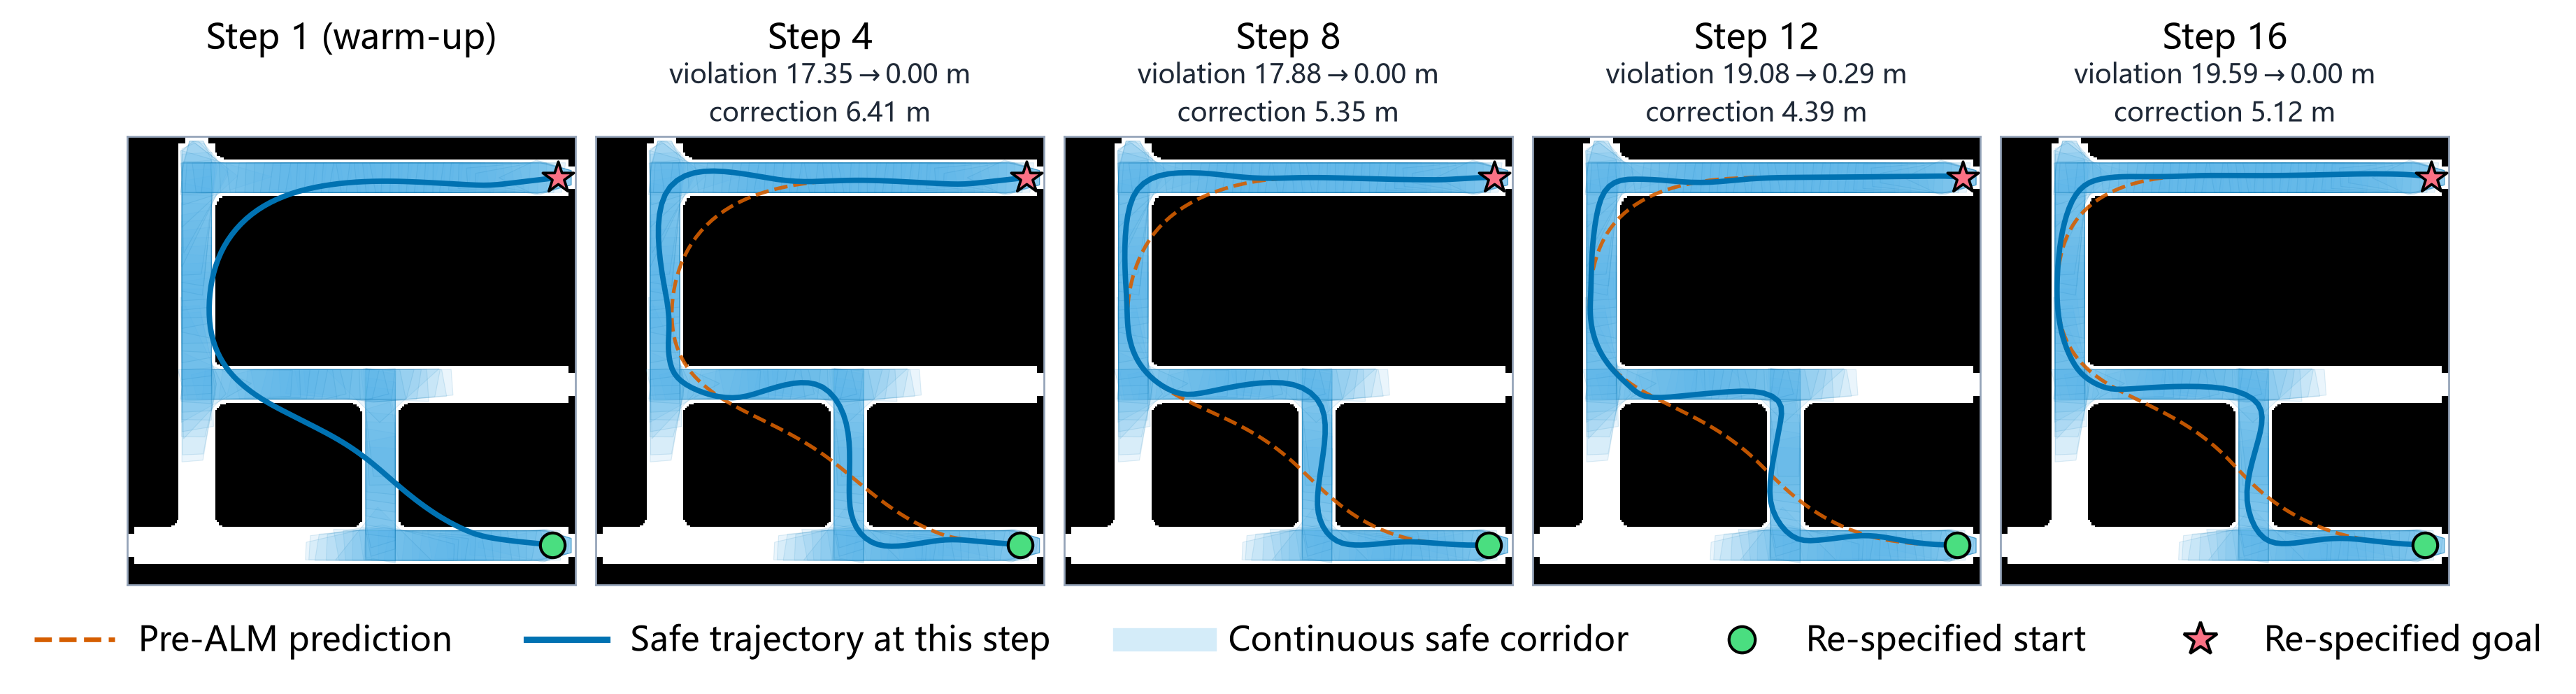
\includegraphics[width=\textwidth]{fig6_diffusion_step_correction.png}
\caption{Trajectory prediction and safety correction during reverse diffusion. The orange dashed line is the prediction before the ALM correction at the current step, the blue curve is the trajectory output at that step, and the light blue region is the safe corridor. The 1st step belongs to the warm-up stage and the corridor is shown for visual comparison only.}
\label{fig:steps}
\end{figure*}

%=====================================================================
\section{Conclusion}
%=====================================================================

This paper proposes TrajSafe-Diffuser, a diffusion-based motion planning method under generative safety constraints. The method guides local safety geometry prediction by task-relevant routes and combines it with a deterministic geometric construction to generate a convex safe corridor, thereby realizing the automatic construction of safety constraints. By incorporating safety latent features into the conditioned denoising network and by using the B\'ezier convex hull property together with the augmented Lagrangian method to enforce constraints on the continuous trajectory, the generated trajectory can take both motion planning accuracy and safety feasibility into account. In addition, the safety correction result is used both for the diffusion state update and for the historical feedback, so that the subsequent denoising process can continuously exploit the available safety correction information.

Experimental results show that the proposed method can effectively reduce trajectory collisions and constraint violations and, while maintaining the trajectory quality, lower the computational cost by reducing the number of sampling steps and sharing convex safe regions. Future work will further study the generation of safety constraints in dynamic environments and incorporate robot kinematics, dynamics and control execution errors in order to improve the applicability of the method in real robotic systems.

%=====================================================================
\bibliographystyle{IEEEtran}
\bibliography{references}

\end{document}
